\documentclass[../../Aurora C# unofficial manual.tex]{subfiles}

\begin{document}
	\section{Adding stars}\label{2_adding_stars}
	Original post can be found
	\href{http://aurora2.pentarch.org/index.php?topic=8495.msg118727#msg118727}{here}.
	\\\\
	
	Adding a new star is straightforward. You click Add New Star. The dialog below pops up and allows you to select spectral class, orbital distance, bearing and parent star.
	\begin{figure}[H]
		\centering
		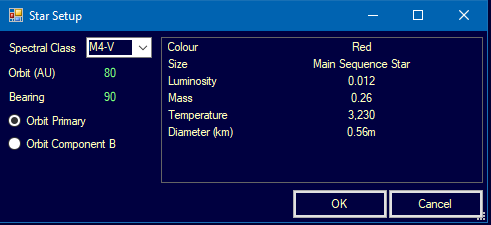
\includegraphics[width=0.5\linewidth]{images/AddingStar}
		\caption[Adding Star]{Adding Star}
		\label{fig:addingstar}
	\end{figure}
	
	This screenshot shows the result of adding the above star to the Alpha Centauri system. New stars do not have any planets or other system bodies. These are added separately and will be covered in a future post.
	\begin{figure}[H]
		\centering
		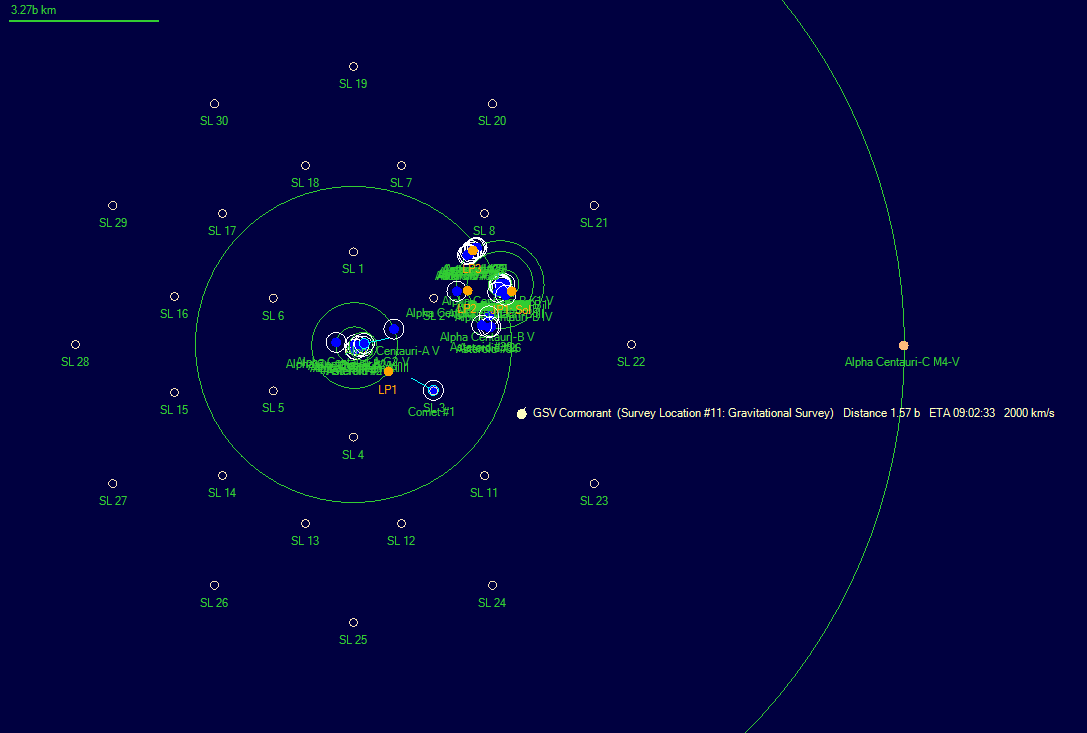
\includegraphics[width=0.95\linewidth]{images/AddingStar2}
		\caption[Adding Star Result]{Adding Star Result}
		\label{fig:addingstar2}
	\end{figure}
\end{document}